\documentclass{aa}  

%
\usepackage{graphicx}
\usepackage{txfonts}
\usepackage{amsmath}
\usepackage{mathrsfs}
\usepackage{booktabs}
\usepackage{tikz}
%\usepackage{hyperref}

%\usepackage[options]{hyperref}
% To add links in your PDF file, use the package "hyperref"
% with options according to your LaTeX or PDFLaTeX drivers.
%

\begin{document} 

   \title{Brute Force Gravitational N Body Simulation - On Stability of Lagrange
   Point Orbits}
   
   \subtitle{Project III - Computational Astronomy}

   \author{Rui Peixoto}

   \institute{Departamento de Física e Astronomia, Faculdade de Ciências,
     Universidade do Porto}

%   \date{Received September 15, 1996; accepted March 16, 1997}

% \abstract{}{}{}{}{} 
% 5 {} token are mandatory
 
  \abstract
  % context heading (optional)
  % {} leave it empty if necessary  
   {}
  % aims heading (mandatory)
   {An algorithm for studying N body astronomical systems is developed and
     applied to the study of the stability of orbits around Lagrange points in
     the solar system.}
  % methods heading (mandatory)
   {A brute force gravitational N body code is discussed. We employ a high
     level language implementation of brute force N body, taking full advantage
     of broadcasting and vectorization to easily optimize the code for a small
     number of bodies. Other possibilities are discussed.}
  % results heading (mandatory)
   {We analyze the stability of perturbations on Lagrange point orbits. We use
     numerical results to give example of stable orbits and discuss their
     applications for satellite orbit.}
  % conclusions heading (optional), leave it empty if necessary 
   {}

   \maketitle
%
%-------------------------------------------------------------------

\section{Introduction}

The many body gravitational problem is a remarkable example of the limitations
of even the most advanced methods in classical mechanics. While the two body
system has an analytical solution, it would take no more than three bodies to present
historical difficulties to the likes of d'Alembert and Poincarré, who struggled
greatly to prove closed form analytical solutions were impossible. Only in 1912
would Sundman discover a solution in series form, albeit of little use, for its
slow convergence.

Astronomical systems, however, are the perfect example of the importance of the
study of many body gravitational systems. Numerical methods are for this reason
crucial to the study of these.

\section{Computational Methods}

\subsection{Code Philosophy}

Out algorithm aims to optimize:

\begin{itemize}
\item Readability and ease of use
\item Optimization for low body count
\item Modular and adaptable structure
\end{itemize}

We achieve this taking advantage of scientific libraries for high level
languages (\textit{numpy} and \textit{scipy}}) which facilitate the use of
vectorization and broadcasting with minimal effort.

\subsection{Implementation}

Brute force approach equates to solving the system of ODE (equations
\ref{eq:setup1} and \ref{eq:setup2})

\begin{equation}
  \label{eq:setup1}
  \frac{d r^k}{d t} & = 2 v^k \\
\end{equation}

\begin{equation}
  \label{eq:setup2}
  \frac{d v^k}{d t} & = - 4 \sum_{i \neq j}^{N} m_j \frac{r_j^k - r_i^k}{|r_j^k - r_i^k|^3} = -4 \sum_{i \neq j}^{N} m_j \Lambda_{ij}^k
\end{equation}

for dimensionless quantities as defined in \cite{monteiro_sebenta_2019}
(conversion factors listed in equations \ref{eq:r_mass} to \ref{eq:r_a}) and
$\Lambda$ of the $k$-th component of the acceleration cause by the $i$-th particle on the $j$-th particle.

Typical scales are defined to be the sum of masses and R the larges radius of
the system.

\begin{equation}
  \label{eq:r_mass}
  m_{r}=M
\end{equation}

\begin{equation}
  \label{eq:r_R}
  r_{r}=R
\end{equation}

\begin{equation}
  \label{eq:r_t}
  t_{r}=\left(\frac{8 R^{3}}{G M}\right)^{1 / 2}
\end{equation}

\begin{equation}
  \label{eq:r_v}
  v_{r}=\left(\frac{G M}{2 R}\right)^{1 / 2}
\end{equation}

\begin{equation}
  \label{eq:r_a}
  a_{r}=\frac{G M}{R^{2}}
\end{equation}

Constructing $\Lambda$ is expensive in terms of memory, but completely avoids
slow high level cycles and expensive non static structures. This step
constitutes the main limitation on the size of the system the algorithm is able
to handle.

Using an adaptative Runge-Kutta 4 integrator with a fittingly small maximum
integration step\footnote{Determining the maximum integration step is generally done in
  an iterative manner. Considering the variation in energy with time one may
  choose a parameter such that energy is conserved.} we get the
time evolution of the system.

\subsection{Collisions}

We avoid the numerical problems related to collisions by substituting equation
\ref{eq:setup2} for equation \ref{eq:collisions} for a small $\epsilon$ when the two
particles are very close.

\begin{equation}
  \label{eq:collisions}
  \frac{d v^k}{d t} & = - 4 \sum_{i \neq j}^{N} m_j \frac{r_j^k - r_i^k}{|r_j^k - r_i^k|^3 + \epsilon} 
\end{equation}

This is suiting for our small number of particles. For a larger number of
particles another options would be to ignore the interaction with particles of a
given proximity, effectively turning off the interaction and allowing particles
to go through each other.

\subsection{Alternative approaches to N body simulations and scaling}

For simulations of more particles one could employ more suited approaches for such
endeavor.

Firstly, one would run into scaling problem in the calculation $\Lambda$, due to
memory limitations.\footnote{Note that $\text{dim} \Lambda = 3N^2$.}. Then now
would do great to take advantage of a lower level language, and cycle over
particles, still employing vectorization but only doing calculations of
dimension $3N$. These algorithms, along with the ones used in our work, scale
with $\mathcal{O}(n^2)$.

For larger scale problems, a more sophisticated approach would be to use
branching algorithms such as Barnes Hut method, which divides space into a grid,
using a tree-searching algorithm to calculate only close interactions and
estimating further ones. With this construction one would be able to bring the
scaling down to a $\mathcal{O}(\log n)$ method. Details about this
implementation can be found in \cite{iwasawa_implementation_2019}.

\section{Code Validation}

\subsubsection{Sun, Earth and Mars}
\label{sec:sun_earth_mars}

Aiming to validate our code we simulate a triple system with circular orbits
with parameters of the Sun, Earth and Mars.

To aid visualization we represent the system in the center of mass reference. We
can see the orbits are stable, as expected, in figure \ref{fig:sun_earth_mars}.

In figure \ref{fig:sun_earth_mars_energy} one may see if our integration is
adequately precise for sufficiently small integration step.\footnote{We see
  that for a large integration energy is not conserved.}

The energy fluctuations happen as energy is exchanged between potential and
kinetic energy, but no net loss is observed.

\begin{figure}
  \centering
  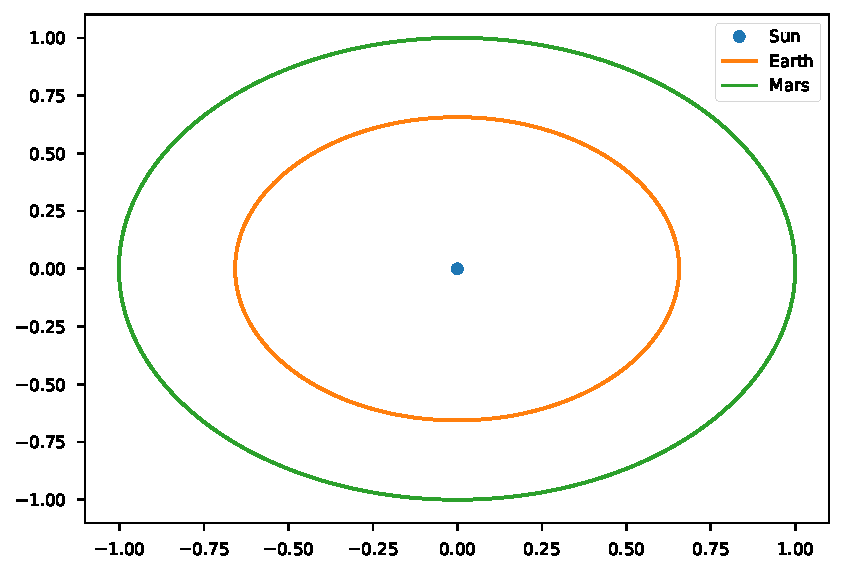
\includegraphics[width=\linewidth]{figs/sun_earth_mars_orbs.pdf}
  \caption{Orbits of circular Sun-Earth-Mars system}
  \label{fig:sun_earth_mars}
\end{figure}

\begin{figure}
  \centering
  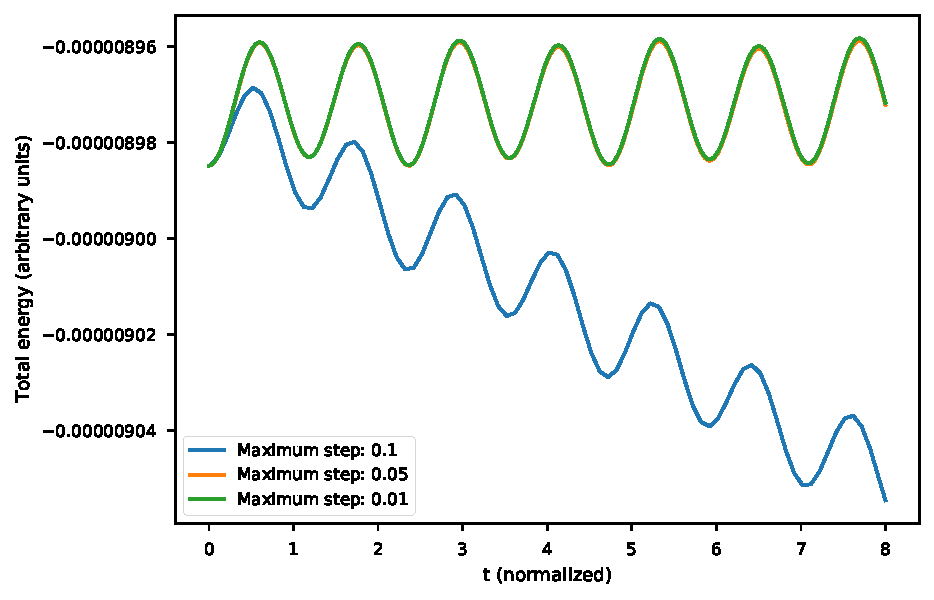
\includegraphics[width=\linewidth]{figs/sun_earth_mars_energy.pdf}
  \caption{Energy dissipation in Sun-Earth-Mars system with step size}
  \label{fig:sun_earth_mars_energy}
\end{figure}


\subsubsection{Sun, Earth and Moon}
\label{sec:sun_earth_moon}

Studying the system Sun-Earth-Moon we validate the capability of our method to
simulate more intricate orbits of hierarchical mass.

Once again employing a circular orbit for the Earth, we see Moon's orbit
crossing Earth's (see figure \ref{fig:sun_earth_moon}) 12 times in one
period around the Sun, in confirmation of our expectations.

\begin{figure}
  \centering
  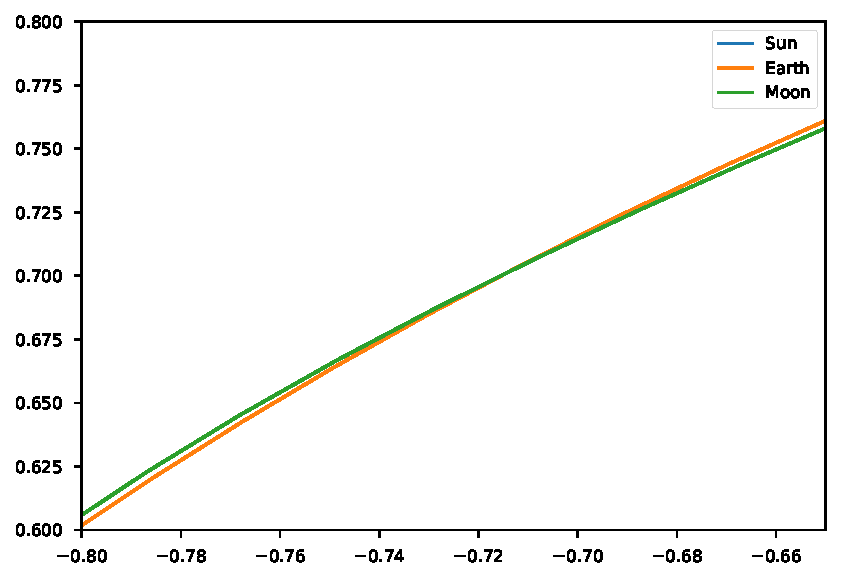
\includegraphics[width=\linewidth]{figs/sun_earth_moon.pdf}
  \caption{Orbital motion of Earth and Moon around Sun}
  \label{fig:sun_earth_moon}
\end{figure}

\begin{figure}
  \centering
  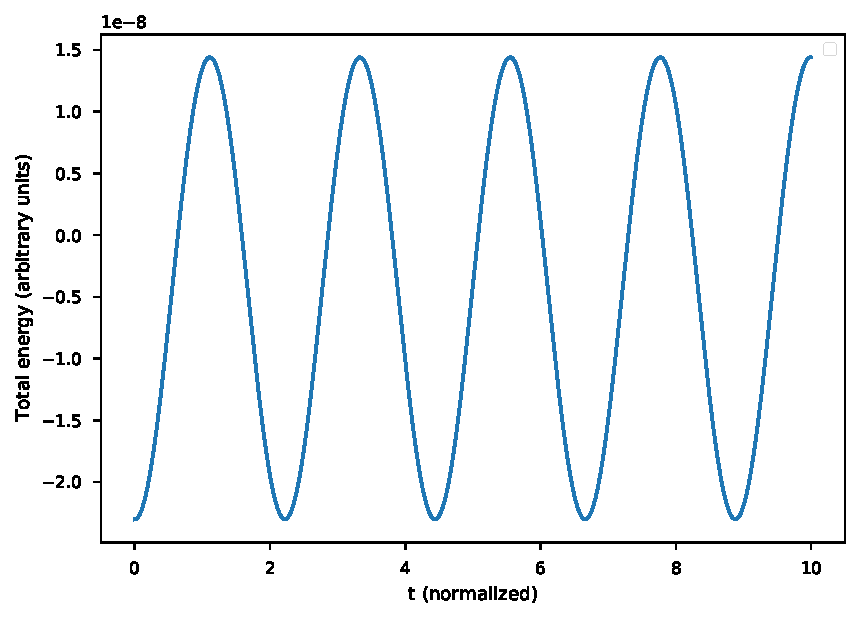
\includegraphics[width=\linewidth]{figs/sun_earth_moon_energy.pdf}
  \caption{Total energy in the Sun-Earth-Moon system}
  \label{fig:sun_earth_moon_energy}
\end{figure}

From figure \ref{fig:sun_earth_moon_energy} we see no dissipation of energy with
time, a reassuring sign that our integration step is sufficiently small.


\section{Application: Stability of Lagrange Points}

We aim to study the stability of orbits around Lagrange points. From \cite{todoran_elliptical_1992} one
concludes that there is an equivalence between Lagrange points in elliptical
orbits and in circular orbits. We will therefore focus our study in the simpler
2D circular case.

The Lagrange points, represented in \ref{fig:lagrange_points}, are
configurations in a hierarchical three body system where the total force on the third object,
smaller than the first two, is so that it will maintain its position relative to
the other bodies.

Lagrange points are extremely useful in astronomy, as they allow astronomers to
place observation and measurement instruments in stable positions in stable
orbit, minimizing difficulties such as fuel cost and target exposure time.

\begin{figure}
  \centering
  \begin{tikzpicture}
    \draw (0, 0) circle [radius=3];
    \draw [dashed] (-3, 0) -- (4, 0);
    \draw [dashed] (0, 0) -- (1.5, 2.6);
    \draw [dashed] (0, 0) -- (1.5, -2.6);
    \draw (1, 0) arc (0:60:1);
    \node at (1, .8) {$\frac{\pi}{3}$};
    \path [fill=orange] (0, 0) circle [radius=.2];
    \path [fill=blue] (3, 0) circle [radius=.15];
    \path [fill=red] (4, 0) circle [radius=.1] node [anchor=south west]{$L_2$};
    \path [fill=red] (2, 0) circle [radius=.1] node [anchor=south east]{$L_1$};
    \path [fill=red] (1.5, 2.6) circle [radius=.1] node [anchor=south west]{$L_4$};
    \path [fill=red] (1.5, -2.6) circle [radius=.1] node [anchor=north west]{$L_5$};
    \path [fill=red] (-3, 0) circle [radius=.1] node [anchor=south east]{$L_3$};
  \end{tikzpicture}
  \caption{Lagrange points}
  \label{fig:lagrange_points}
\end{figure}

There are five points in an orbit that follow this conditions, but not all of
them are stable. Stable orbits are possible around $L_4$ and $L_5$ points, where
the Coriolis effect acts as a restoring force. $L_1$, $L_2$ and $L_3$,
however, do not allow for stable orbits. To verify these results we study
Lagrange points $L_1$ and $L_5$ in a circular Sun-Earth like system for a
satellite-like object (parameters in table \ref{}).

\begin{table}
  \centering
  \begin{tabular}{c|c|c|c}
    \toprule
    Parameter & Sun & Earth & Satellite \\ \midrule
    Mass (kg) & 1.989 \times 10^{30} & 5.972 \times 10^{24} & (1 \times 10^3 / 1 \times 10^{14}) \ \  \footnote{Both values are used in each analysis, verifying the orbits are stable for a wide range of masses.} \\
    \bottomrule
  \end{tabular}
  \caption{Sun-Earth-Satellite parameters}
  \label{tab:params}
\end{table}

\subsection{Lagrange point $L_1$}
\label{sec:l1}

One may compute the conditions for $L_1$ by solving the quintic equation
\ref{eq:l1} for the distance to the Earth-like object $r$, where $M_1$, $M_2$,
$R$ are the masses of the Sun-line object, the Earth-line object and the radius
between them, respectively.

\begin{equation}
  \label{eq:l1}
  \frac{M_{1}}{(R-r)^{2}}=\frac{M_{2}}{r^{2}}+\frac{M_{1}}{R^{2}}-\frac{r\left(M_{1}+M_{2}\right)}{R^{3}}
\end{equation}

Because $M_1 << M_2$ one could approximate $r$ by the Hill sphere's radius, as
in equation \ref{eq:hill_l1}.

\begin{equation}
  \label{eq:hill_l1}
  r \approx R \sqrt[3]{\frac{M_{2}}{3 M_{1}}}
\end{equation}

However, when we do so, we see the approximation is not good enough for the
Sun-Earth system, as can be seen in figure \ref{fig:l1_unstable}, where we do not get a stable orbit.

\begin{figure}
  \centering
  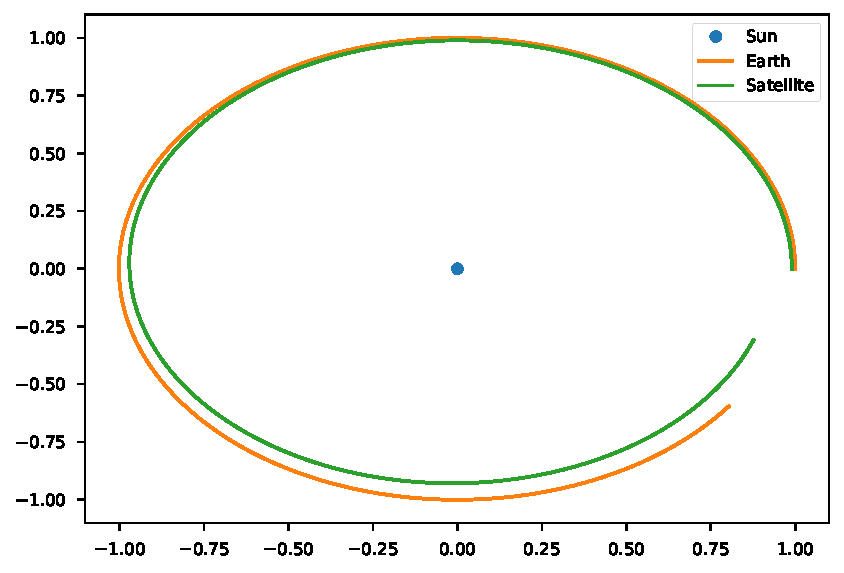
\includegraphics[width=\linewidth]{figs/l1_unstable.pdf}
  \caption{Unstable orbit for approximate $L_1$}
  \label{fig:l1_unstable}
\end{figure}

Using a consecutive bisection method to numerically solve equation \ref{eq:l1}
will however provide us with a stable orbit (see figure \ref{fig:l1_stable}).

\begin{figure}
  \centering
  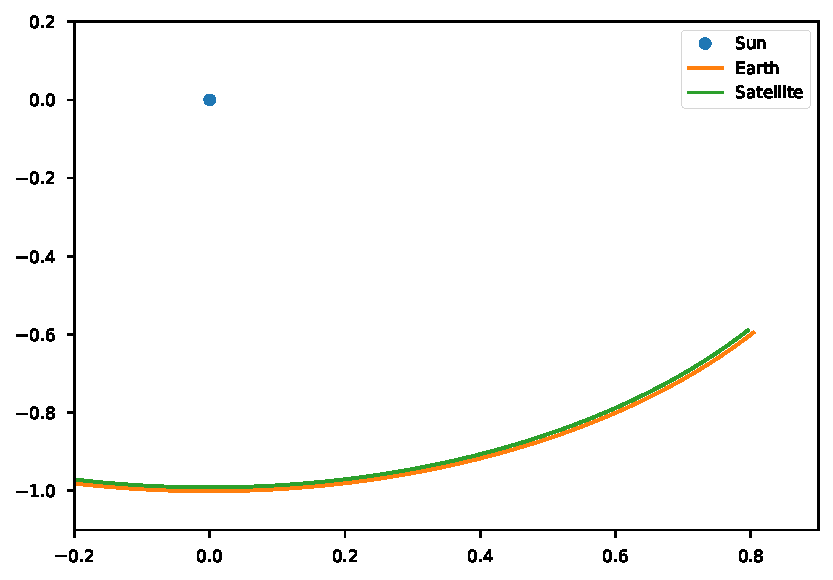
\includegraphics[width=\linewidth]{figs/l1_stable.pdf}
  \caption{Stable orbit around $L_1$}
  \label{fig:l1_stable}
\end{figure}

In figure \ref{fig:l1_relative_r} we can see the variation of the relative radii
of Satellite-like object with time for small perturbations of the form $r' = r (1 + b)$. It is clear that
even for very relatively small perturbations the orbit rapidly becomes unstable,
transitioning to a non radially stationary orbit.

Additionally, we verify that the movement of the Satellite-like object does not
depend on its mass, as long as it preserves the system's hierarchy.

\begin{figure}
  \centering
  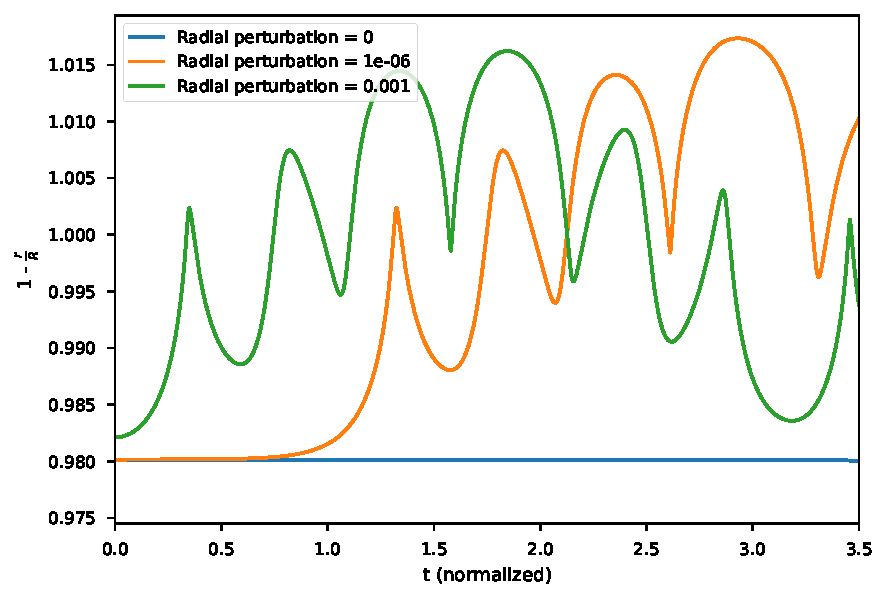
\includegraphics[width=\linewidth]{figs/l1_radius_perturbation.pdf}
  \caption{Relative radii of the Satellite-like object with perturbations}
  \label{fig:l1_relative_r}
\end{figure}

\subsection{Lagrange point $L_5$}

Lagrange point $L_5$ lies in the trajectory of the Earth-like object, with a
phase difference of $-\frac{\pi}{3}$. In this case, the initial conditions of
the Satellite-like object can be determined analytically with simple vector projection.

The evolution of this system can be seen in figure \ref{fig:l5_orb}.
Additionally, if a radial perturbation is introduced (see
\ref{fig:l5_radial_perturbation}), we see a very different behavior than that of
the $L_1$ orbit. Instead of the divergent behavior we see for a perturbation in
the radius like in the first case, we now see an oscillatory behavior.

\begin{figure}
  \centering
  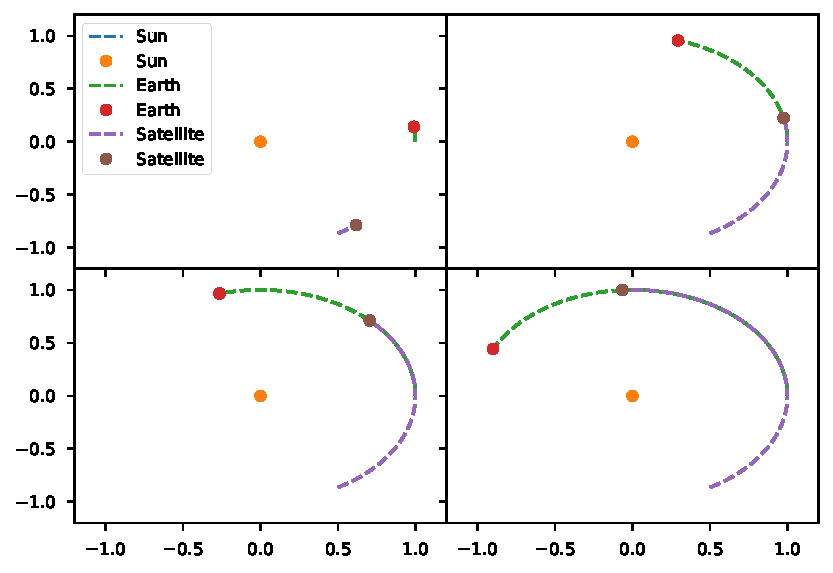
\includegraphics[width=\linewidth]{figs/l5_orbit.pdf}
  \caption{Evolution of Sun-Earth-Satellite-like system in $L_5$ orbit (left to
    right)}
  \label{fig:l5_orb}
\end{figure}

\begin{figure}
  \centering
  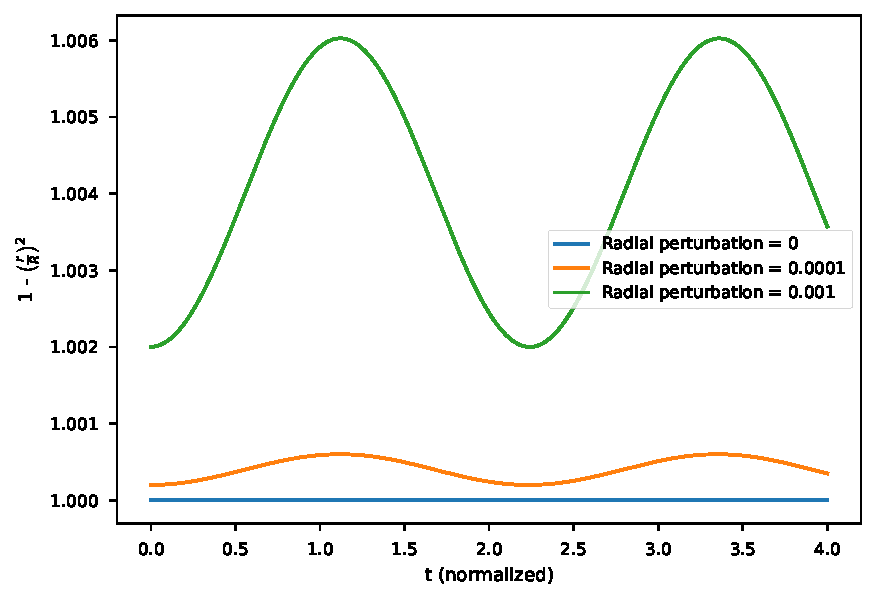
\includegraphics[width=\linewidth]{figs/l5_radius_perturbation.pdf}
  \caption{Radial perturbation in $L_5$ orbit}
  \label{fig:l5_radial_perturbation}
\end{figure}

This is a consequence of having a stable orbit. Another difference is that a
radial perturbation will not significantly alter the period (for $b <
0.2$), like it does in the case of the $L_1$ point. This is clear when we
represent the trajectory for a perturbed radius in figure \ref{fig:l5_perturbed_orb}.

\begin{figure}
  \centering
  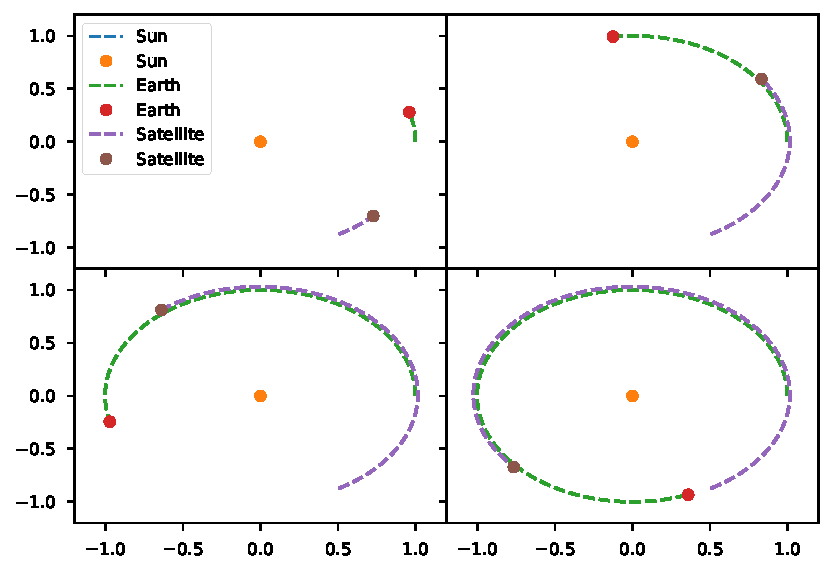
\includegraphics[width=\linewidth]{figs/l5_pert_orbit.pdf}
  \caption{Orbit of $L_5$ with a radial perturbation $b \approx 0.01$}
  \label{fig:l5_perturbed_orb}
\end{figure}

\subsection{Possible orbits around Lagrange points}

\subsubsection{Oscillations around $L_1$}

While effectively less stable, Lagrange points $L_1$, $L_2$ are extremely
important because they constitute the best position to observe solar, earthly
and outer solar system phenomena, simultaneously providing ease of communication
back to observatories.

However, a satellite on the precise Lagrange point is directly obstructing the
Sun-Earth-outer solar system line of sight. To allow for multiple instruments in
conflict free positions and to avoid line of sight problems, semi-stable orbits
around these points are utilized.

One simple example of such orbit, at $L_1$, may be obtained by giving the
Satellite-like object's position a $z$ component. The planar orbit is not
significantly changed, but now we see the object oscillates in the $z$ axis, as
can be seen in figure \ref{fig:l5_z}.

\begin{figure}
  \centering
  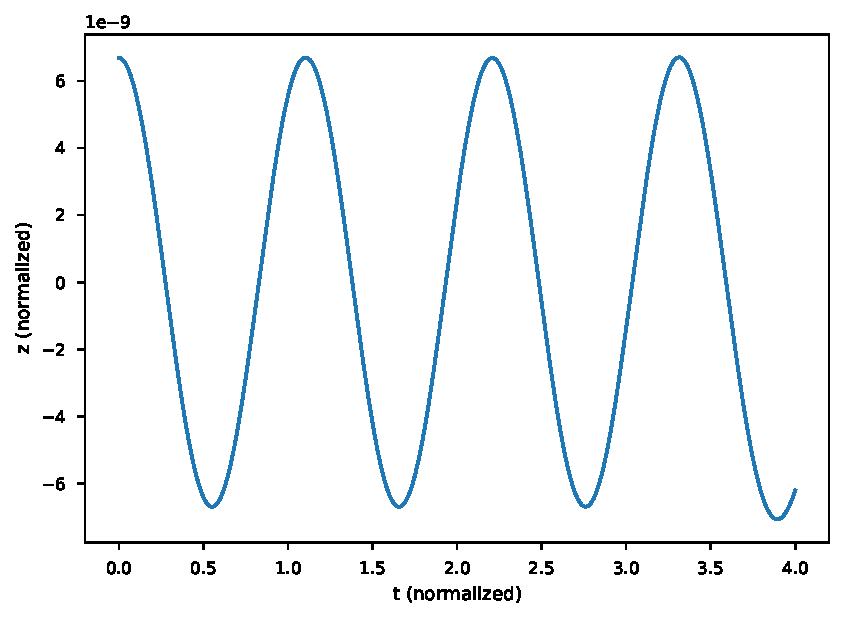
\includegraphics[width=\linewidth]{figs/l5_z.pdf}
  \caption{$z$ oscillations around orbit $L_1$ in stable regime}
  \label{fig:l5_z}
\end{figure}

These orbits, along with other more complex (with slight periodic corrections,
which form the know Lissajous orbits), allow for a much more efficient and
practical use of this astronomical real-estate.

\subsubsection{Influece of Jupiter on $L_5$ stability}

Including another large body on the simulation, in this case, a Jupiter-like
body, we see (figure \ref{fig:l5_jup}) the stability of the orbit is broken and
oscillations are induced.


\begin{figure}[h!]
  \centering
  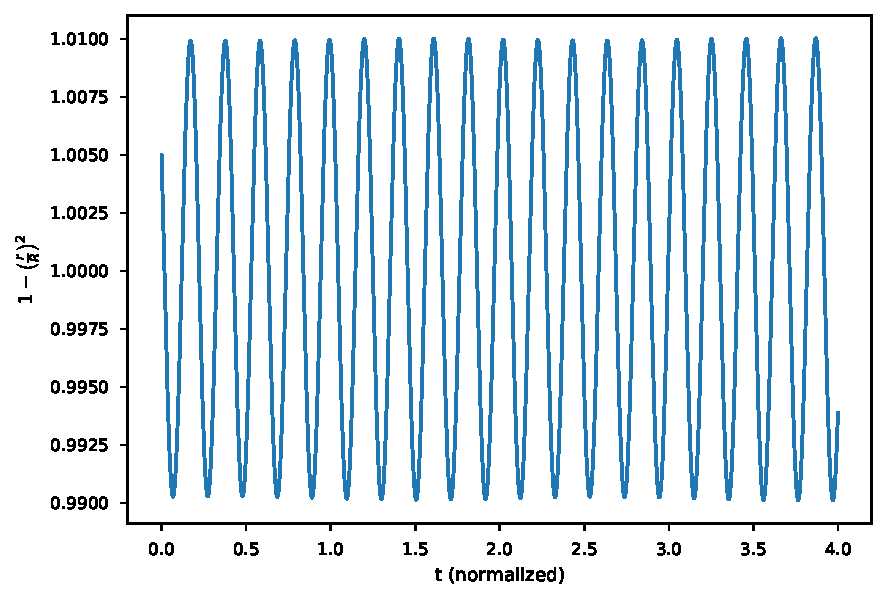
\includegraphics[width=\linewidth]{figs/l5_d_jup.pdf}
  \caption{Radial flutuations cause by Jupiter-like object on $L_5$ orbit}
  \label{fig:l5_jup}
\end{figure}

This effect means that even the stable orbits of $L_4$ and $L_5$ require a given
amount of orbit compensation.

\newpage

\section{Conclusion}

\begin{itemize}
\item An efficient, high level, understandable brute force gravitational N body
  code was developed for small systems.
\item Algorithm was validated for the circular Sun-Earth-Mars and Sun-Earth-Moon systems.
\item N body method was applied to the study of Lagrange points
\item Considerations were made about the stability of orbits around $L_1$ and
  $L_5$ points.
\item Stability of $L_5$ orbits and instability of $L_1$ orbits were confirmed
  and simulated.
\item Confirmed the need for numerical solution for the quintic equation for $L_1$ radius determination.
\item Studied the influence of Jupiter on the $L_4$ and $L_5$ orbits.
\item Discussed the importance of Lagrange points and practical orbits around
  even unstable points are possible with minimal trajectory correction.
\end{itemize}

\begin{acknowledgements}
  This work was done under the orientation of professor Mário João Monteiro in the
  context of the curricular unit of Computational Astronomy.
\end{acknowledgements}

\bibliographystyle{aa}
\bibliography{nbody}

\end{document}